\section{Measurement method and checking the tools}
\label{sec:method}

\paragraph{Changes to the code.} All our changes are compile-time switches in
\texttt{src/pe\_opts.h}. Without them the code behaves like the original \gapbs. The only
change in the default build is that every \texttt{\#pragma omp parallel for} is split into
\texttt{parallel} and \texttt{for}, which does the same thing. With the switches we can turn on
PAPI regions inside every parallel region (the PAPI high-level API only counts the thread
that calls it), the edge counter, \texttt{schedule(runtime)}, prefetching, huge pages,
parallel first touch, relabelling and other values of $\alpha$ and $\beta$. A script builds 27
variants, and every variant has to pass the BFS verifier of \gapbs{} (\texttt{-v}) before we
time it.

\paragraph{How we time.} For every configuration we first do one run that we throw away, and
then 5 runs of 24 searches each. The sources of the searches are chosen pseudo-randomly, but
they are the same for all variants and both machines. We use the timer of \gapbs{} around
one search. Inside one run the first searches are slow (Figure~\ref{fig:warmup}): on Hábrók
the first five take between 99 and \SI{156}{ms}, and after that about \SI{4}{ms}. So we drop
searches 1 to 5 of every run, which leaves 95 samples per configuration. As in the lectures,
we report the median and the interquartile range (IQR) in ms per search, and GTEPS $=
m/t_\text{median}$. The IQR is between \SI{14}{\percent} (Hábrók, kron22) and
\SI{56}{\percent} (laptop, kron20) of the median. We only call a difference significant if it
is bigger than the IQR of both configurations.

\begin{figure}[ht]
\centering
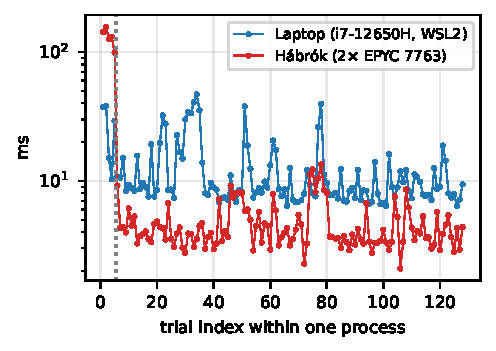
\includegraphics[width=0.55\linewidth]{figures/warmup.pdf}
\caption{Time of every search inside one run (128 searches, log scale). The slow first
searches on Hábrók and the outliers on the laptop are the reason why we drop searches 1 to 5
and use the median.}
\label{fig:warmup}
\end{figure}

\paragraph{Checking the tools.} Before we use a tool, we want to know that it measures the
right thing. Table~\ref{tab:validation} shows our checks.
\begin{table}[ht]
\centering\small
\caption{Checks of the measurement tools.}
\label{tab:validation}
\begin{tabular}{@{}p{3.4cm}p{6.1cm}p{4.6cm}@{}}
\toprule
Check & Result & Conclusion \\
\midrule
Timer resolution & \texttt{CLOCK\_MONOTONIC}: \SI{1}{ns}, one call takes \SIrange{34}{36}{ns} & small compared to a search (more than \SI{1}{ms}) \\
Wall time from 3 tools (laptop, 64 searches) & \gapbs{} load + searches \SI{0.679}{s}, perf \texttt{duration\_time} \SI{0.717}{s}, \texttt{/usr/bin/time} \SI{0.69}{s} & they agree, the \SI{38}{ms} difference is starting the program \\
CPU time from 2 tools & perf task-clock \SI{6.00}{s}, \texttt{time} user + sys \SI{6.05}{s} & within \SI{1}{\percent} \\
pecount against perf & page faults \num{36422} and \num{36423} & pecount gives the same result \\
gprof & \SI{100}{\percent} of the samples in \texttt{frame\_dummy} & \textbf{not usable} for OpenMP: it does not assign the time of the OpenMP threads to the right functions \\
perf sampling & BUStep, InitParent and TDStep are found; libgomp has no symbols but is found by library & reliable \\
PAPI against pecount (Hábrók, 1 thread, 64 searches) & sum of the 5 PAPI regions divided by pecount: cache misses \SI{99.1}{\percent}, references \SI{97.2}{\percent}, cycles \SI{95.0}{\percent}, instructions \SI{90.3}{\percent} & they agree, the rest is code outside the regions (last loop, bitmap resets) \\
Known result: integer loop (PAPI) & \num{5.000} instructions and \num{4.000} cycles per iteration & the loop has 5 instructions, \texttt{imul} (3 cycles) + \texttt{add} (1 cycle) \\
Known result: pointer chase over \SI{1}{GB} (PAPI) & \num{1.0007} cache misses per step & one miss per random load, as expected \\
Known results with pecount & loop: \num{4.99} instructions per iteration; chase: \num{2.4} misses per step & counters were shared (multiplexed), and the scaling is wrong when the program has phases, so we use PAPI regions \\
Timers on Hábrók & \texttt{/usr/bin/time} is not installed & cross-check only on the laptop \\
\bottomrule
\end{tabular}
\end{table}

\paragraph{The verifier found a data race.} Running the verifier on every variant was useful.
With \texttt{schedule(runtime)} and \texttt{OMP\_SCHEDULE=dynamic,100} or \texttt{guided},
\emph{every} search gave a wrong BFS tree (0 of 8 correct on both machines), and
\texttt{static,1000} was wrong in 4 of 8 searches on the laptop and in all 8 on Hábrók. The
reason is that \texttt{BUStep} sets bits in the shared \texttt{next} bitmap with a normal,
non-atomic read-modify-write of a 64-bit word. This is only safe when the block of every
thread starts at a word boundary, so when the chunk size is a multiple of 64. The original
\texttt{dynamic,1024} fulfils this without saying so. Plain \texttt{static} passed our tests,
but only by luck, because its blocks also do not have to start at a word boundary. In the
schedule experiments we therefore only used chunk sizes that are a multiple of 64.
